\chapter{Additional for Dissertation}
\thispagestyle{empty}
\emph{The last chapter containing some additional things needed for a complete 
dissertation document required for a promotion at the University of Groningen.}
\null
\vfill

\begin{myexampleblock}{Parts of this chapter are adapted from:}
  \authors{Caroline Durrant, Morris A. Swertz, Rudi Alberts, Danny Arends, ... , Ritsert C. Jansen, Klaus Schughart, et al}\\
  \emph{ Bioinformatics tools and database resources for systems genetics analysis in mice 
         - a short review and an evaluation of future needs}\\
  \bold{Briefings in Bioinformatic} (2011)\\\\
\end{myexampleblock}

\newpage

\section*{Conclusion, Discussion and Future perspectives}
\addcontentsline{toc}{section}{Conclusion, Discussion and Future perspectives}
This chapter will highlight the major conclusions of this thesis. There will be a short 
discussion on the implications of these conclusions.  Finally there will be a short future 
perspectives part, in which we look forwards to the future of high throughput computing in 
systems genetics. We highlight some novel innovations since the previous chapters were 
written, and outline possible issues which might become more relevant to systems genetics 
research in the coming years.

\subsection*{Multiple QTL mapping and interaction models}
Association and / or linkage analysis will continue to be the bread-and-butter analysis 
tool-set for systems geneticists of the future. However complex systems geneticists have 
to cope with the aquisition of data from diverse experimental designs and the analysis of 
these diverse data types. Requiring complex pipelines to analyse new complexity of the incoming data.

In chapter \ref{sect:Metabolites} we compare three different experimental designs: full 
block design, random design and generalized genetical genomics (GGG) design design. We show 
that using a GGG experimental design for experiments gives higher statistical power to 
detect interactions between environmental and genetic variation compared to a random. 
Additionally the amount of raw data produced in this design is 4 times less compared to 
a full block design, making the post analysis of these kind of experiments less challenging, 
and less expensive.

Another part of this complex pipeline is the association analysis part which can be performed using 
different methods, e.g. single marker association mapping in outbred populations, interval 
mapping in inbred populations, or multiple QTL mapping. In this thesis we used multiple 
QTL mapping to find QTLs for classical traits related to germination of seeds in 
\emph{A. thaliana}, shows the an increase in QTL detection power of MQM versus standard 
single marker QTL mapping. This shows that more genetic loci are involved in germination 
of seeds then previously known.

Furthermore, we have shown the application of interaction models to multi environmental 
experiments in which we used a generalized genetical genomics experimental design. We 
conclude that interaction models are a very powerful tool in understanding the complex 
interplay between genetics and (cellular) environments. Additionally, we observe more QTLs 
are detected by using a designGG experimental design compared to a random design.

\subsection*{High throughput analysis}
With increasing scale of experimental data being produced in the lab, it will not be 
sufficient to have analysis software as simple downloads, because the researcher will 
also need sizable compute and storage power \cite{Schadt:2010}. Thus, researchers will 
need easy access to 'software as a service' such as cloud computing. 

How this increasing demand for raw computational power can be satistfied in the future remains 
an unanswered question. Although federate computing providers (such as Target or EUgrid) can help 
researcher in their need for big computing solutions in the near future. This is also not a 
universal solution, while the speed of data production is currently higher then the speed of 
CPU improvement. Two solutions which are currently already available are highlighted here: 
Cluster and cloud computing might be able to solve the Big Data questions researchers face 
now-a-days.

\subsubsection*{Cluster computing}
A cluster is a collection of computers dedicated to solving a computational task by divide 
and conquer. It basically means to having a basic relatively homogeneous software available 
on demand, on suitable compute and storage hardware. Hardware resources are divided by an 
internal scheduling system amongst different tasks form different users. Users in general 
have little control over the computational environment, because administration of the cluster 
and the scheduling system put contraints on the usage of cluster. Computing clusters can be 
fashioned from different types of hardware, such as:
\begin{itemize}
  \item Ad-hoc networks Cheap FPGA, and ARM core
  \item Dedicated computer clusters, PBS
  \item Video card cluster for linear algebra
\end{itemize}
Compute clusters in general do not have to be homogeneous in nature. Though in many cases 
there will be some homogeneity to provide users with a stable computational environment to 
perform their tasks. Additionally the use of hardware can limit the usage of a cluster to a 
certain range of computational tasks.

\subsubsection*{Cloud computing}
The term cloud is used in many different ways. It basically means to have software available 
on demand, on suitable compute and storage hardware, with the user being charged for the time 
that it is being used. Following the concept of the leading cloud provider Amazon, it refers 
in practice to use of a virtual Linux machine, i.e. a virtualized compute server with Linux 
pre-installed, hosted within some large compute infrastructure, with complete freedom to be 
customized by the user although not for free\cite{Trelles:2011}.

Many commercial, national and local compute centres are also increasingly providing computer
server capacity in cloud fashion. This makes these virtual machines an easy method to distribute 
software without the need for users to install software. Thus, the infrastructure is specified
jointly but for the actual computation every partner can be private with their data. This 
approach grants enormous computational power to everyone with minimal preparation - once that 
a shared image is finalized.

The setup of such a compute cloud is not trivial but several initiatives are underway to ease 
this process. At the workshop, the Bioinformatics WG tested the packaging system provided by 
the Debian Med initiative as a method to create a cloud and could be consider this as a seed 
for an image to then be publicly shared. Instructions to create such images were prepared for 
the workshop and made available at:\\
 http://wiki.debian.org/DebianMed/LiveCD. 
 
Using this method the cloud infrastructure can be transferred to local computer clusters 
if desired. Every participant has access to the server and can grant access to collaborators 
without having to pay the hosting fees. When complete, this server image can be ported to 
cloud providers such as: Amazon, Rackspace to be reused by other researchers.

\subsection*{Git and SVN - software code sharing and versioning}

Access and sharing of software code of all aforementioned tools is essential to avoid 
duplication of efforts, promote interoperability and to really collaborate within the mouse 
genetics bioinformatics community. Only then does it really become clear what is available 
and how there can be data and software flow between projects.

An example tool to facilitate such sharing and collaboration on code level is Git: Git 
allows users to follow updates (versions) of software packages and easily provide feedback. 
The most recent stable R version of R/qtl and qtlHD can be found as a Git repository, Git 
helps to control versions for the authors and facilitate compatibility with other packages 
such as QTL-bim and Pheno2Geno. Although most users will generally find the last stable version 
(Git master branch) the most useful and user-friendly, it is possible to download a 
development branch to get familiar with the new features being prepared for the next version.

An alternative to Git is Subversion. (SVN). GeneNetwork code was developed using Subversion with 
Python as its primary language. GeneNetwork code and a shell (partial) database are available on 
Source Forge:\\
http://sourceforge.org/projects/genenetwork

The mapping and permutation code used by GN for real time analysis is based on fast 
Haley-Knott approximations and is available on Source Forge:\\
http://qtlreaper.sourceforge.net

xQTL and XGAP code were also developed in Subversion using Java as its primary language and 
R for its analysis interfaces. XGAP code and binaries are all available as open source at
http://www.xgap.org and http://www.molgenis.org. From a developer's perspective both Git and
SVN are equally well-suited for publishing code and may be used in parallel. However recently 
in 2012 also the entire MOLGENIS software suite (MOLGENIS, XGAP, xQTL workbench) was transfered 
to Git and moved to http://www.github.com to get more online exposure, and remove the need 
to host an internal SVN server.

Additionally, all software developed described in this thesis was also written and developed 
using git for source code control. And is available from Github at:
http://github.com/DannyArends/

\section*{Future Perspectives}
In the future, further considerations should include integration of mapping analysis tools 
with genomic annotation and sequence data. Another goal should be the generalization of 
analysis frameworks to accommodate not only mouse and human data but also data from model 
species with different genetic pedigree structures, such as pets (e.g. dogs), farm animals
(e.g. horses, cattle, pigs) and plants (e.g. arabidopsis, brassica, maize). 

\subsection*{Pheno2Geno}
Generating bio markers from micro array and RNAseq data is possible using mixture models, 
additionally Pheno2Geno provided highly optimized routines for generating genetics maps 
de-novo or to saturate existsing genetic maps. Its output structures are compatible with 
R/qtl, which provides many facilities for QTL mapping in inbred populations.

With the upcoming new version of R/qtl also the pheno2geno package needs to be redesigned 
to accomodate new requirements. These include expected changes such as: a more standalone package, 
further optimization of parallelisation, but also support for more cross types such as 
diversity outbred and/or collaborative cross mice. But also other more uncertain requirements 
which might or might not come up: E.g. One of the main developer of pheno2geno is currently working 
on polyploid species. Due to this investment of the first author in polyploid crops such as 
potatoes and tomatos, we also expect to see basic support for this in upcoming versions of 
the pheno2geno package. The authors are also committed to maintaining the package, and source 
code is available as open source code making it easier to support future new requirements.

\subsection*{xQTL workbench}
While the xQTL workbench system described in this thesis have the ability to absorb new 
analysis methods, consideration should be given to allow high flexibility. It will be very 
difficult to anticipate totally new demands and requirements, or even new developments 
which could provide a better alternative than databases for data and R for analysis. xQTL 
workbench is a framework that incorporate appropriate mechanisms to support new demands and 
developments.

There is a need for reliable but flexible infrastructure in systems genetics. xQTL workbench 
combines, the flexibility of the MOLGENIS suite with some of the most used computational tools 
for systems genetics. Together with R as esparanto between the different languages, this creates 
a system which systems geneticists can use to keep track of data generation and track their analysis. 
Using R as computational backend allows them to contribute their methods and algorithms back to 
the scientific community.

\subsubsection*{wormQTL and wormQTL - Human Disease}
The current version of WormQTLHD (August 2013) is a comprehensive and compendious database that 
enables molecular model organism data to be studied in the context of human diseases. Just as with 
WormQTL \cite{Snoek:2012}, we believe that WormQTLHD will be continuously curated by the members of 
the \emph{C. elegans} community. The results of the 'broad-sweep' disease-enrichment test in 
combination with the web tool will be of special interest to researchers in the human or worm 
domain. We believe these results could also be applied to prioritize the pathogenic variants 
increasingly being produced by next-generation sequencing in diagnostic labs. Genetic variants 
affecting human genes of unknown function may have worm orthologues that are part of human-worm 
phenologs and these may reveal or imply a role in a human disease. Thus, through functionally 
conserved networks, missing information can be inferred and candidate genes can be selected via 
model organisms.

The approach of WormQTLHD is conceptually similar to that described by Smedley et al. 
\cite{Smedley:2013}. They created an automated method called PhenoDigm to provide evidence about 
gene–disease associations by analysing phenotypic information. In their case, phenotypes consist of 
a collection of ontology terms, which are aligned and scored to derive an overall phenotype-similarity score. Using this 
method, known gene–phenotype associations in model organisms (mouse, zebrafish) can be transferred 
to other organisms such as man, and help us to understand the genetic cause of disease. This method 
works best when the model organism is physiologically close to man and has comparable classical 
phenotypes. It would therefore be less useful for \emph{C. elegans}. However, combining the molecular 
(WormQTLHD) and phenotypical (PhenoDigm) approaches may result in a very powerful tool to discover 
novel gene–disease associations in man, especially when using physiologically close model organisms.

We plan to further develop the WormQTLHD data and toolset. There might be more ways in which 
researchers would like to search through the large amounts of data, for example, based on custom 
lists of gene identifiers, or by combining tools such as finding QTLs within specific regions. 
The QTL plots could be improved or replaced with interactive graphs that are more informative and 
would allow the users to continue 'drilling down' in the data instead of returning to the home page 
for a new analysis with a different tool. Furthermore, we envisage close integration with other data 
sources and tools such as WormNet, R/qtl and GO Enrichment to provide even more biological context 
and analytical tools for the user.

Our new database makes this data attractive and easy-to-use for an even wider community of 
quantitative geneticists working on worms and man. We are committed to maintaining the data and 
software in the future and invite the community to add and share their new data and ideas. 

\subsection*{R/qtlHD}
Because of increasing data sizes, R might not be the most suitable platform for the analysis 
of next generation high throughput data. While the R environment is well suited to scientific 
computing and performing statistical analysis, it is not the fastest or most optimized 
language available. When dealing with high throughput data obtained from RNA-seq, exome sequencing 
or Bi-sulfite sequencing data sizes quickly become the limitation for any software package 
written in R. Because R/qtl-HD is aimed at QTL analysis of high-density, high-throughput data, 
R is not a suitable language for the computation parts fo the algorithm.

R/qtlHD is written in the high performance D programming language. D is chosen as primairy language 
because it is created to perform safe and high throughput numerical analyses using a C like syntax. 
This C style syntax provides a familiar syntax for people with a C/C++ background. Additional features which according 
tot the R/qtl development team make D the language f choice include:
\begin{enumerate}\itemsep1pt
\item \emph{Improve code quality} - This makes the code more maintainability and more readable code is 
easier to reason about and optimize leading to improve performance of algorithms.
\item \emph{D allows to call C} D allows to call C (and a limited subset of C++) functions directly. This 
allows to re-use previously written R/qtl code (which was written in R and C).
\item \emph{Unittesting} Unittesting is build into the D programming language, allowing programmers to use the 
power of unit- and regression testing to build a test suite without the need for external 
frameworks
\item \emph{Concurrency and Actors} - The D language provides high level patterns such as Actors and 
Message Passing to deal with parrallelization of code. Unlike other languages, this is a build in 
feature of the language
\item \emph{Static typing} D requires types to be known at compile time, this reduces the risk for 
run-time errors of the system.
\item \emph{Compile Time Function Execution} Compile time function execution is a feature that allows 
building look up tables at compile time. This has the opportunity to greatly reduce the run time of 
algorithms, by pre-calculating common cases.
\end{enumerate}
There are more reasons for the R/qtl development team to favor D, however these are less tangible then 
the above mentioned reasons.

The current version of R/qtl provides many tools for genetic map construction, but also several historical 
methods for QTL mapping. R/qtl-HD will not provide a multitude of methods but focus more on the high speed 
analysis of data using stable and proven methods. such as Haley-Knott regression and analysis of variance.
Additional features such as genetic map construction and validation are not high priority when converting 
the current software into a more optimized language. R/qtl-HD mains to mapping huge volumes of traits onto 
medium to large genetic maps.

Additionally the multiple QTL mapping (MQM) routines from R/qtl will also be converted into the D programming language.
The MQM routine has proven to be a useful addition to the R/qtl toolkit and with the new implementation of R/qtl as 
R/qtlHD, we aim to improve the usefulness even more. The major limitation in MQM is the additional computational 
load when compared to single marker QTL mapping. The R/qtl development team is committed to 1) add the Multiple QTL 
Mapping routine to the R/qtlHD package and 2) provide further optimization to MQM to allow it to handle even large 
volumes of trait and genetic data.

An overview of the features planned for the R/qtl-HD package:
\begin{enumerate}\itemsep1pt
\item \emph{Universal input format} - Based on our experiences with XGAP and xQTL workbench, QTAB was developed as input 
                                      format for Rqtl-HD. A testing version of QTAB was implemented in R/qtl-HD by Pjotr 
                                      Prins. The QTAB format aims to provide a universal solution to the storage of genotype 
                                      and genetic maps in inbred populations.
\item \emph{Single marker QTL mapping} - R/qtl HD aims to provide the most common single marker mapping methods. These methods 
                                         will be optimized to work with huge amounts of phenotype data, created by new technologies 
                                         such as tilling arrays, RNA-seq and/or exome sequencing.
\item \emph{Multiple QTL mapping} - We aim to implement multiple QTL mapping and as such benefit from the added advantages of the D 
                                    language such as: Reduced memory usage during runtime and less run time due to the fact that 
                                    it is easier to use parrallel computation in D.
\item \emph{R interface} - Current R/qtl users should be able to switch to R/qtl-HD, while keeping their familiar R interface. in 
                           an ideal world current users should automatically switch to R/qtl-HD without them noticing
\item \emph{BioRuby} - Bio-packages are being created for many languages (Python, Perl, etc), Ruby is a new and upcoming language in the 
                       scientific field. R/qtl HD aims to provide bindings to the BioRuby project as as proof of concept, other BioPackages 
                       could model their own bindings on these ruby bindings
\item \emph{Compatibility} - R/qtl-HD aims to be compatible with the following operating systems: Mac OS X, Microsoft Windows and Debian Linux.
\end{enumerate}

R/qtlHD is developed as open source community software, currently a very limited version is available as preview for
download. To download a development version, go to Github: http://github.com/qtlHD/qtlHD

\newpage

\section*{Dutch Summary}
\addcontentsline{toc}{section}{Dutch Summary}
Systems genetics is the inter disciplinairy field which deals with the consequences of genetic 
variation on a biological system. The goal of systems genetics is to partition this variation 
into three major categories: Genetic, Environment and Error variation, and explain how complex
phenotypes arise from a combination of these three major factors.  Natural variation (or 
genetic pertubation) is used to interogate the genetic component of phenotype variation. 
Combined with environmental pertubation we can investigate the influence different 
environments and the interaction between genetics and environment. Experimental design and 
statistics are used to minimize and estimate error variance.

Pheno2Geno (Chapter 2) deals with the creation of genetic maps from large scale omics data. 
The theory of genetic map construction is ~100 years old. Software available for genetic map 
construction has not been adapted yet to make use of new technologies such as multi threading 
or cluster computing. Pheno2Geno aims to provide analysis of data from tilling arrays or RNAseq 
to generate gene based expression markers and create high density genetic maps.

Chapter 3 describes the implementation of the Multiple QTL mapping routine by R. C. Jansen into 
R/qtl. Adding a 'new' algorithm to the R/qtl toolset which aims to provide a range of QTL 
mapping tools for inbred crosses. R/qtl is the basis of a toolset build around a unified 
data structure allowing easy adaptation and extension of the software. R/qtl allows researchers 
to analyse data from different sources or to quickly compare different approaches.

In chapter 4 we show case our ideas for a generic storage and computation platform for systems 
genetics. Our demo system xQTL workbench is currently being used as a backend to the 
WormQTL and WormQTL-HD database. xQTL workbench allows users to store and share their data in 
a local or web environment, and run analysis across datasets using the power of distributed 
computing. It comes standard with QTL mapping tools such as: R/qtl, PLINK and qtlbim but also
provides a web inferfaces, data importers, APIs and visualizations.

Current work on using differences in correlation to generate interaction networks and detect 
cell type specific QTL effects is described in chapter 5. Correlated Traits Locus analysis 
(or CTL mapping) enables researchers to find genetic loci controlling correlation differences 
in segregating phenotypes. A variation on this method has proven valuable in discovering cell 
type specific eQTL effects. These effects can be used to untangle cell mixtures seen in whole 
blood gene expression data.

%In short this proposed method creates a proxy for cell counts in an unrelated cohort. this proxy 
%is then used during meta analysis as artifical cell count across many different cohorts. The 
%interaction effects between QTL and Proxy are used to assign a cell type to each eQTL. In the final 
%stage diseases in which cell type enrichment is prominent are tested by using publicly available data.

Last we have some additional required chapters, such as this summary in Dutch, a CV and publication 
list and bibliography.\\

I hope you enjoy reading this thesis as much as I enjoyed creating it during the last four years,\\\\

Danny Arends (Aug 2013)

\newpage
\section*{Abbreviations and Acronyms}
\addcontentsline{toc}{section}{Abbreviations and Acronyms}
{\footnotesize
\begin{tabular}{ l l }
API:         & Application Programming Interface\\
BC:          & Backcross \\
bp:          & Base pair(s) \\
cM:          & centi Morgan \\
CPNN:        & Collaborative computing project for NMR\\
CSV:         & Comma separated values\\
CTL:         & Correlated traits locus \\
DesignGG:    & Experimental design of genetical genomics software\\
DRY:         & Principle of don't repeat yourself\\
DSL:         & Domain Specific Language\\
EBI:         & European Bioinformatics Institute\\
FINDIS:      & Finish disease database\\
GEMs:        & Gene expression based genetic marker\\
GEN2PHEN:    & EU project to unify human and model organism genetic variation databases\\
GMOD:        & Generic model organism database project\\
GUI:         & Graphical user interface\\
GWAS:        & Genome Wide Association Study\\
GWL:         & Genome Wide Linkage analysis\\
HGVBaseG2P:  & Human genome variation database of genotype-to-phenotype information\\
HTML:        & Hypertext markup language\\
IDE:         & Integrated Development Environment\\
JAR:         & Java Software Archive\\
LGPL:        & Lesser general public license\\
MAGE-TAB:    & Microarray gene expression tab delimited file format\\
Mbp:         & Mega base pairs = 1.000.000 bp \\
MOLGENIS:    & Molecular genetics information systems toolkit\\
NordicDB:    & Nordic Control Cohort Database\\
OBF:         & Open Bioinformatics Foundation\\
OntoCAT:     & Ontology common API toolkit\\
PEAA:        & Patterns for enterprise application architecture\\
QTL:         & Quantitative trait locus\\
RDF:         & Resource description format\\
REST:        & Representative state transfer web services\\
RIL:         & Recombinant inbred line \\
SNP:         & Single Nucleotide Polymorphism\\
SOAP:        & Simple Object Access Protocol\\
SQL:         & Structured Query Language\\
UML:         & Uniform data Modeling Language\\
WAR:         & Web Application aRchive file\\
XML:         & Extensible Markup Language\\
XGAP:        & Extensible genotype and phenotype software platform. 
\end{tabular}
}
\newpage

\section*{Acknowledgements}
\addcontentsline{toc}{section}{Acknowledgements}
Knowledge is in the end based on acknowledgement\\
- Ludwig Wittgenstein (1889 - 1951)\\\\

There are many people who need to be thanked and acknowledged, 
here are the people who made the cut:

{\bf Ritsert C. Jansen} to whom I owe my life in science, thank you for giving 
me this chance to work in your group and develop my skills in research and 
education. {\bf Anna Mulder} my girlfriend for all the times I left you and 
{\bf Oscar} (our cat) for my science endavours. Thank you for your trust in 
me and giving me a home to come home to. {\bf Pjotr Prins} Always forgotten, Never 
Ignored. All the people past and present at the {\bf Groningen BioInformatics Centre} 
(GBIC) group for putting up with me. {\bf Yang Li} for your mentorship and all 
the vibrant discussions we had at GBIC, {\bf Joeri v/d Velde} my friend and coworker 
for all the good times hacking on Java and R in Haren. My student {\bf Konrad Zych} 
for his dedication and help with chapter \ref{chap:pheno2geno}. {\bf Morris Swertz} 
my co-promotor, you were a great help when writing chapter \ref{chap:xqtlwormbench} 
and always made me feel at home at GCC. Also all the guys from the {\bf Genomics Coordination 
Centre} (GCC) department for all the End of Sprints, presentations, discussions and beers. 
{\bf Lude Franke} and {\bf Harm-Jan Westra} for the very informative collaboration on the 
human GWA study (chapter \ref{sec:cellspecificeqtl}), I learned a LOT from you, and am 
extremely thankful for your help with the final chapters of this thesis. {\bf Wilko ligterink}, 
{\bf Henk Hilhort} and {\bf Ronny Joosen} for doing the \emph{Arabidopsis thaliana} 
experiments, and trusted me to analyze their data. I learned a lot especially about 
the more 'bio' parts of this thesis. The {\bf University of Groningen} (RUG) for 
educating me and providing me with an place to do my research. Finally the {\bf 
University Medical Centre Groningen} (UMCG) for the pleasant working atmosphere 
and good lunches.

\newpage

\section*{About the author}
\addcontentsline{toc}{section}{About the author}
\subsection*{Curriculum Vitae}
\addcontentsline{toc}{subsection}{Curriculum Vitae}

\begin{wrapfigure}{r}{0.4\textwidth}
  \centering
  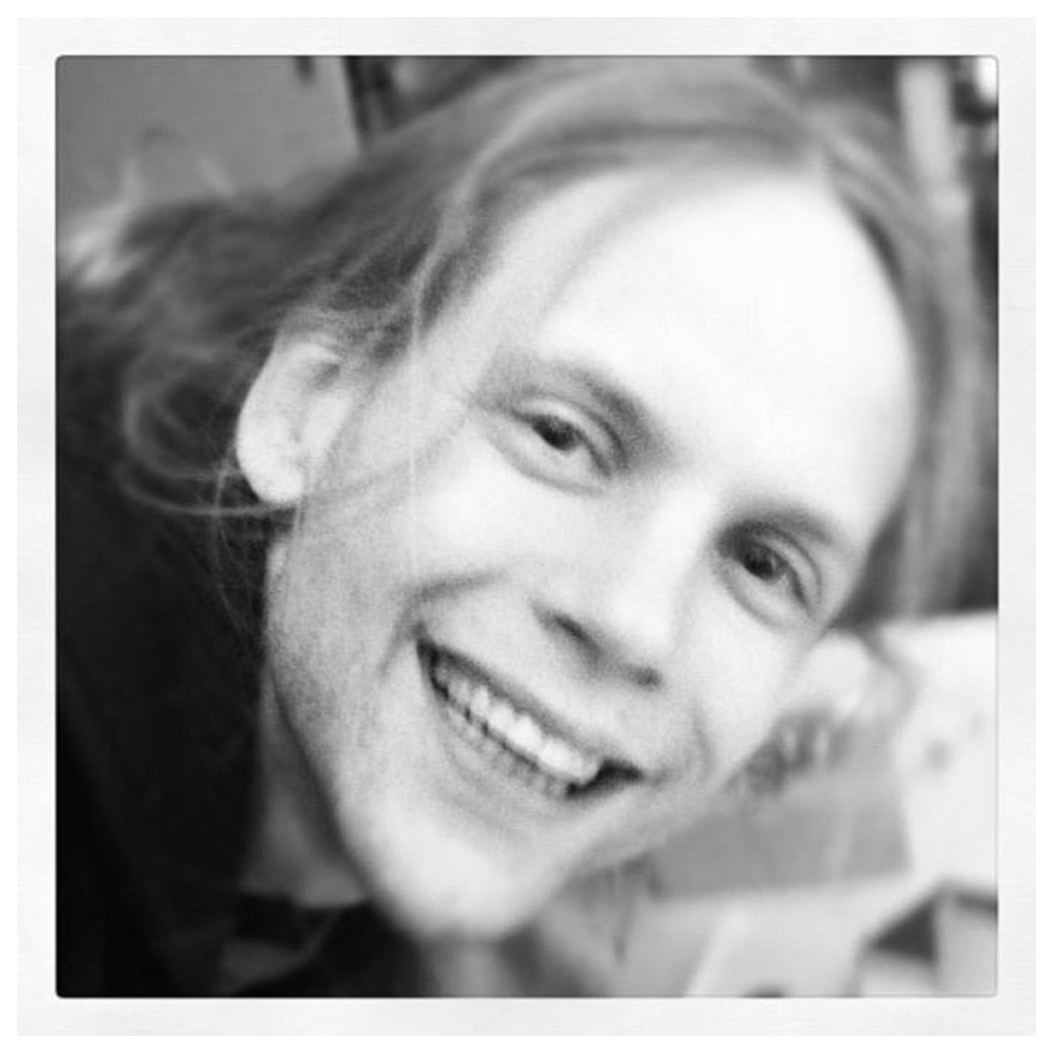
\includegraphics[width=0.3\textwidth]{eps/image_6_1.eps}
\end{wrapfigure}

Danny Arends was born on the 15th of Juli 1983 in the city of Zwolle located in the heart 
of the Netherlands. After moving twice, Danny went to an elementary school situated in 
Heiligerlee, a minuscule hamlet in the north of Holland in the province of Groningen. 

The small school was a perfect match for young Danny during his childhood. Here he quickly 
fell in love with mathematics, and the wondrous world of numbers and patterns. With the 
advent of computers at the elementary school, the love for computers and their inner 
workings also began to develop.

Heiligerlee is located next to a small forest called 'De Hoogte', this forest was used 
by Danny and friends on a daily basis to build tree huts and by using snow balls in winter 
wage war on kids from the other school in Heiligerlee. The forest combined with growing up 
amidst animals on a farm-like residence sparked young Danny his intrests in biology.

After elementary school Danny went to the Ubbo Emmius lyceum in Stadskanaal (Groningen). 
The large scale VWO was a big change from the small elementary school. Long hours at school 
together with a long bus ride to and from school, made for long days. Fortunately new 
friends were made in the class room and during the long bus rides. Danny finished high 
school after 6 years, taking mostly exact courses such as mathematics, physics and chemistry.

At 17, A university degree should be the next step in his career. Because of his interests 
in computers, Danny decided that computer science would be a good match. This turned out 
to be not so true. While deeply intrigued by the subject of computational machines, He 
was not satisfied by just studying the workings of a machine build by man.

After two years of Computer science at the University of Groningen, Danny decided it was time 
for a change. Computer science was replaced by Life Science \& Technologie, a bachelor which 
was recently formed as a collaboration between the Biology faculty and Medical Sciences.

He finished his bachelor in record tempo, partly due to the exemptions obtained from 
doing two years of computer science. A Master in molecular biology was quickly selected after
being introduced to bioinformatics at GBIC during a previous bachelor project. The molecular 
biology master allowed for customization of the courses followed, and bioinformatics became the main 
theme in all of the master theses produced. The first thesis: "Machine learning to predict 
transcriptional regulation in prokaryotes" was produced in the group of Oscar Kuipers. 
The second "R/QTL, MQM algorithm" was done in the lab of Ritsert C. Jansen.

Parts of this second master thesis are also in this thesis (chapter \ref{chap:mqm}).
After finishing his master Cum Laude, a PHD was started with Ritsert C. Jansen at the 
Groningen Bioinformatics Centre with a focus on the use of bioinformatic tools to handle 
current challenges in genetics and statistics. The four years of research at GBIC have 
lead to the thesis you are currently reading.\\\\

\newpage

\subsection*{List of Publications}
\addcontentsline{toc}{subsection}{List of Publications}

\subsection*{Authored:}
   R/qtl: high throughput Multiple QTL mapping\\
  \authors{Danny Arends*, Pjotr Prins*, Ritsert C. Jansen and Karl W. Broman}\\
  \bold{Bioinformatics} (2010)\\\\
  Visualizing the genetic landscape of Arabidopsis seed performance\\
  \authors{Ronny V. L. Joosen*, Danny Arends*, Leo Willems, Wilco Ligterink, 
           Henk Hilhorst and Ritsert C. Jansen}\\
  \bold{Plant Physiology} (2011)\\\\
  xQTL workbench: a scalable web environment for multi-level QTL analysis\\
  \authors{Danny Arends*, K. Joeri van der Velde*, Pjotr Prins, Karl W. Broman, 
           Steffen Moller, Ritsert C. Jansen and Morris A. Swertz}\\
  \bold{Bioinformatics} (2012)\\\\
  WormQTL: Public archive and analysis web portal for natural variation data in Caenorhabditis spp\\
  \authors{L. Basten Snoek*, K. Joeri Van der Velde*, Danny Arends*, Yang Li*, 
           Antje Beyer, Mark Elvin, Jasmin Fisher, Alex Hajnal, Michael O 
           Hengartner, Gino B. Poulin, Miriam Rodriguez, Tobias Schmid, 
           Sabine Schrimpf, Feng Xue, Ritsert C. Jansen, Jan E. Kammenga 
           and Morris A. Swertz}\\
  \bold{Nucleic Acids Research} (2012)\\\\
  Identifying genotype-by-environment interactions in the metabolism of germinating Arabidopsis seeds 
  using Generalized Genetical Genomics\\
  \authors{Ronny V. L. Joosen*, Danny Arends*, Yang Li*, Leo Willems, Joost J. B. Keurentjes, Wilco Ligterink, 
           Ritsert C. Jansen, Henk Hilhorst}\\
  \bold{Plant Physiology} (2013)

\subsection*{Co-Authored:}
  The MOLGENIS toolkit: rapid prototyping of biosoftware at the push of a button\\
  \authors{Morris A Swertz, Martijn Dijkstra, Tomasz Adamusiak,  Joeri K van der Velde, 
           Alexandros Kanterakis, Erik T. Roos, Joris Lops, Gudmundur A. Thorisson, 
           Danny Arends, George Byelas, Juha Muilu, Anthony J. Brookes, Engbert O. de Brock, 
           Ritsert C Jansen and Helen Parkinson}\\
  \bold{BMC Bioinformatics} (2010)\\\\
  XGAP: a uniform and extensible data model and software platform for genotype and phenotype experiments\\
  \authors{Morris A Swertz, K. Joeri van der Velde, Bruno M Tesson, Richard A Scheltema, 
           Danny Arends, Gonzalo Vera, Rudi Alberts, Martijn Dijkstra, Paul Schofield, 
           Klaus Schughart, John M. Hancock, Damian Smedley, Katy Wolstencroft, Carole 
           Goble, Engbert O. de Brock, Andrew R Jones, Helen E Parkinson and Ritsert C Jansen}\\
  \bold{Genome Biology} (2010)\\\\
  SYSGENET: a meeting report from a new European network for systems genetics\\
  \authors{Klaus Schughart, Danny Arends, P. Andreux, R. Balling, Pjotr Prins, et al.}\\
  \bold{Mammalian Genome} (2010)\\\\
  Trans-eQTLs Reveal that Independent Genetic Variants Associated With a Complex Phenotype Converge on 
  Intermediate Genes, with a Major Role for the HLA\\
  \authors{Rudolf SN Fehrmann, Ritsert C. Jansen, Jan H. Veldink, Harm-Jan Westra, Danny Arends,
           Marc Jan Bonder, Jingyuan Fu, Patrick Deelen, Harry J. M. Groen, Asia Smolonska, 
           Rinse K. Weersma, Robert M. W. Hofstra, Wim A. Buurman, ... , Lude Franke}\\
  \bold{Plos Genetics} (2011)\\\\
  Bioinformatics tools and database resources for systems genetics analysis in mice - a short review 
  and an evaluation of future needs\\
  \authors{Caroline Durrant, Morris A. Swertz, Rudi Alberts, Danny Arends, Steffen Möller, 
           Richard Mott, Pjotr Prins, K. Joeri van der Velde, Ritsert C. Jansen and 
           Klaus Schughart}\\
  \bold{Briefings in Bioinformatics} (2011)\\\\
  WormQTLHD - a web database for linking human disease to natural variation data in C. elegans\\
  \authors{K. Joeri van der Velde*, Mark de Haan, Konrad Zych, Danny Arends, L. Basten Snoek, 
           Jan E. Kammenga, Ritsert C. Jansen, Morris A. Swertz and Yang Li}\\
  \bold{Nucleic Acids Research} (2014)

\subsection*{In Preparation/ Under Review / In Press:}
  Pheno2Geno - High throughput generation of genetic markers and maps from molecular phenotypes\\
  \authors{Konrad Zych, K. Joeri van der Velde, Ronny V. L. Joosen, Wilco Ligterink, Ritsert C Jansen 
           and Danny Arends}\\
  \bold{BMC Bioinformatics} (201X)\\\\
  Correlated Traits Locus mapping\\
  \authors{Danny Arends, Pjotr Prins, Harm-Jan Westra, Yang Li, Lude Franke and Ritsert C. Jansen}\\
  \bold{Unknown} (201X)\\\\
  TiQS: web environment for expression QTL analysis\\
  \authors{Steffen M\"oller, Ren\'e Sch\"onfelder, Hajo Krabbenh\"oft, Benedikt Bauer, Yask Gupta, 
           Pjotr Prins, Danny Arends, et al.}\\
  \bold{BMC Bioinformatics} (201X)\\\\
  Multiple QTL mapping of cardiac collagen deposition in an F2 population of Scn5a mutant mice reveals 
  interaction between Fgf1 and Pdlim3, Gpr158 \& Itga6\\
  \authors{Elisabeth M. Lodder, Brendon P. Scicluna, L. Beekman, Danny Arends, et al.}\\
  \bold{Genome Research} (201X)\\\\
  Regulatory Network of Secondary Metabolism in Brassica rapa: An Insight In The Glucosinolate Pathway
  \authors{Dunia Pino del Carpio, Ram Kumar Basnet, Danny Arends, Ke lin, Ric CH de Vos, Dorotha Muth, 
           Jan Kodde, Kim Boutilier, Johan Bucher, Xiaowu Wang, Ritsert Jansen, Guusje Bonnema}\\
  \bold{Plos One} (201X)

\subsection*{Acknowledged in:}
  DesignGG: an R-package and web tool for the optimal design of genetical genomics experiments\\
  \authors{Yang Li, Morris A Swertz, Gonzalo Vera, Jingyuan Fu, Rainer Breitling and Ritsert C Jansen}\\
  \bold{BMC Bioinformatics}, 10:188 (2009)\\\\
  Generalizing genetical genomics: getting added value from environmental perturbation\\
  \authors{Yang Li, Rainer Breitling and Ritsert C. Jansen}\\
  \bold{Trends in Genetics}, 24:518-524 (2008)

\subsection*{List of Presentations}
\addcontentsline{toc}{subsection}{List of Presentations}
R/xqtl: High throughput modeling, mapping and exploration of Big Data\\
SYSGENET meeting - Braunschweig, April 2010\\\\
Introduction into QTL analysis\\
Dynamic Presentation - University of Groningen, Aug 2010\\\\
MQM and HPC for R/qtl\\
CSBG meeting - Wageningen University, Sept 2010\\\\
Introduction into QTL mapping - Bioinformatics I\\
University of Groningen, June 2011\\\\
(Re)Construction of genetic maps from gene expression data\\
GBIC - University of Groningen, July 2011\\\\
R/qtl for Big Data\\
MIT Department of Biology, invited by Jeroen PJ Saeij\\
MIT, Boston (MA), May 2011\\\\
The Challenge of Big Data Genetical Genomics\\
NCSA, invited by Victor Jongeneel and Chris Fields\\
NCSA, Urbana (IL), May 2011\\\\
Introduction into QTL mapping - Learning From nature (LFN)\\
Wageningen University, Feb 2012\\\\
Computer practical / tutorial - Learning From nature (LFN)\\
Wageningen University, Feb 2012\\\\
Introduction into R and R/qtl\\
Summer Course - King's college, Sept 2013\\\\

\subsection*{List of Posters}
\addcontentsline{toc}{subsection}{List of Posters}
User friendly cluster computing for QTL analysis\\
  \authors{Danny Arends, Joeri v/d velde}\\
  \bold{ISMB} July 2010 - Boston, USA\\\\
Multiple QTL mapping poster\\
  \authors{Danny Arends, Pjotr Prins,Karl W. Broman and Ritsert C. Jansen}\\
  \bold{GBIC day} September 2010 - Groningen, The Netherlands\\\\
Pheno2Geno poster\\
  \authors{Konrad Zych, Danny Arends, Ritsert C. Jansen}\\
  \bold{NBIC} April 2012 - Lunteren, The Netherlands\\\\
Pheno2Geno poster\\
  \authors{Konrad Zych, Danny Arends, Ritsert C. Jansen}\\
  \bold{ECCB / ESCS} Sept 2012 - Basel, Swiss\\\\
GWAS in potato\\
  \authors{Konrad Zych, Danny Arends, Ritsert C. Jansen}\\
  \bold{Kings College} Sept 2013 - London, UK

\subsection*{Awards}
\addcontentsline{toc}{subsection}{Awards}
1st place Poster Award 'Pheno2Geno' at ESCS2012 Basel (Swiss) (2012)\\
Travel Grant by NBIC for ISMB in Boston (MA, USA) (2010)\\
2nd place Poster Award xQTL workbench NBIC Conference (Lunteren) (2010)\\
Travel Grant 'Short course on system genetics' in Bar Harbor (MA, USA) (2009) by JAX laboratory\\
